% % -*- coding:utf-8 -*-
\documentclass[aspectratio=169,10pt]{beamer}
\nonstopmode

\usepackage{appendixnumberbeamer}
\usepackage{graphicx}
\usepackage{url}
\usepackage{pdfpages}
\usepackage{mathtools}
\usepackage{amsmath}
\usepackage{wasysym}
% color palette
\definecolor{tu01}{HTML}{84B818}
\definecolor{tu02}{HTML}{D18B12}
\definecolor{tu03}{HTML}{1BB5B5}
\definecolor{tu04}{HTML}{F85A3E}
\definecolor{tu05}{HTML}{4B6CFC}
\definecolor{tu06}{HTML}{E3B505}
\definecolor{tu07}{HTML}{AF331D}
\definecolor{tu08}{HTML}{000000}
\definecolor{tu09}{HTML}{AAAAAA}
\definecolor{tu10}{HTML}{444444}
\definecolor{tu11}{HTML}{84B818}

% mixed and light colors
\colorlet{tu01light}{tu01!33}
\colorlet{tu02light}{tu02!33}
\colorlet{tu03light}{tu03!33}
\colorlet{tu04light}{tu04!33}
\colorlet{tu05light}{tu05!33}
\colorlet{tu06light}{tu06!33}
\colorlet{tu07light}{tu07!33}
\colorlet{tu08light}{tu08!33}
\colorlet{tu09light}{tu09!33}
\colorlet{tu10light}{tu10!33}
\colorlet{tu11light}{tu11!33}

\colorlet{tu01midlight}{tu01!50}
\colorlet{tu02midlight}{tu02!50}
\colorlet{tu03midlight}{tu03!50}
\colorlet{tu04midlight}{tu04!50}
\colorlet{tu05midlight}{tu05!50}
\colorlet{tu06midlight}{tu06!50}
\colorlet{tu07midlight}{tu07!50}
\colorlet{tu08midlight}{tu08!50}
\colorlet{tu09midlight}{tu09!50}
\colorlet{tu10midlight}{tu10!50}
\colorlet{tu11midlight}{tu11!50}

\colorlet{tu01dark}{tu01!80!black}
\colorlet{tu02dark}{tu02!80!black}
\colorlet{tu03dark}{tu03!80!black}
\colorlet{tu04dark}{tu04!80!black}
\colorlet{tu05dark}{tu05!80!black}
\colorlet{tu06dark}{tu06!80!black}
\colorlet{tu07dark}{tu07!80!black}
\colorlet{tu08dark}{tu08!80!black}
\colorlet{tu09dark}{tu09!80!black}
\colorlet{tu10dark}{tu10!80!black}
\colorlet{tu11dark}{tu11!80!black}

\colorlet{lightgray}{gray!25}
\colorlet{midlightgray}{gray!50}
\colorlet{anthracite}{black!85}

% aliases
\colorlet{tudo}{tu01}
\colorlet{tuorange}{tu02}
\colorlet{tudolight}{tu01light}

% \usepackage{beamerthememetropolis}
\usetheme[progressbar=frametitle,noslidenumbers]{metropolis}
\newcommand{\themename}{\textbf{\textsc{metropolis}}\xspace}


\usepackage{xcolor}



\title{Pr\"asentation Bachelor Arbeit:\\
 Simulation von Online Scheduling-Algorithmen f\"ur parallele Systeme}
% \subtitle{Learning to Identify Similarities between Mathematical Expressions}
\author{Hendrik Rassmann}

\institute{TU Dortmund University - Department of Computer Science}
\titlegraphic{\hfill
\includegraphics[height=8mm]{tu-do-logo.pdf}}

\date{November 02, 2020}

\begin{document}


\maketitle
\Large

\begin{frame}{\"Ubersicht}
\tableofcontents
\end{frame}


\begin{frame}[fragile]{Startpunkt}

\begin{columns}
	\begin{column}{0.57\paperwidth}
		\vspace{0.5pt}
		
\includegraphics[width=\linewidth, clip]{images/Arndt}
	\end{column}
	\begin{column}[c]{0.43\paperwidth}
		\begin{itemize}
			\item \alert{Network}
			\item \alert{Online}
			\item \alert{Experiments} ... \alert{confirm}
		\end{itemize}
	\end{column}
\end{columns}
\end{frame}
\section{Problemstellung}


\begin{frame}[t,fragile]{Problemstellung}
Ausgehend von:

\begin{itemize}[<+->]
	\item Rechner/\emph{Nodes} unterschiedlicher \emph{Geschwindigkeiten} bilden zusammen ein (Rechen)\emph{Cluster} 
	\item Auftr\"age/\emph{Jobs} kommen im laufenden Betrieb rein (\emph{online})
	\item Auftr\"age unterscheiden sich bez. \emph{Bearbeitungszeit}, \emph{Anzahl} an ben\"otigten Knoten und \emph{Ankunftszeitpunkt}
	\item Auftr\"age sollen auf eine 'geeignete' Art und Weise bearbeitet werden
\end{itemize}
\end{frame}


\begin{frame}[t,fragile]{Zielfunktionen \footnote{Kriterien von Arndt. et al.}}
\begin{itemize}[<+->]
	\item \emph{makespan} ''Zeit bis Feierabend''
	\item \emph{average flow time} ''Supermarkt - Nur der Apfel? Gehen Sie doch gerne vor''
	\item \emph{average waiting time} 	
	\item \emph{maximum waiting time} ''Restaurant - Wenn ein Tisch nicht bedient wird, kommen G\"aste nicht mehr wieder''
\end{itemize}
\end{frame}

\begin{frame}[t, fragile]{Scheduling-Algorithmen (Referentiell Transparent)\footnote{Auswahl von Arndt. et al.}} 
$Scheduling$-$Algorithmus : Warteliste \rightarrow Auftrag$\\
\pause

\begin{itemize}[<+->]
	\item First in First out (\emph{FiFo})
	\item Shortest Processing Time first (\emph{SPT})
	\item Greates Processing Time first (\emph{GPT})
\end{itemize}
\end{frame}



%
\includegraphics[page=1, scale=0.4]{SchedulingBeispiel.pdf}
\setbeamercolor{background canvas}{bg=}

\includepdf[pages=2-]{SchedulingBeispiel.pdf}

\begin{frame}[t, fragile]{Scheduling-Algorithmen (Referentiell Intransparent)}
\begin{itemize}[<+->]
	\item Random
	\item \alert{First Fit} (W\"ahle den am l\"angsten wartende Auftrag, der sofort gestartet werden kann)
	\item \alert{Backfilling} (W\"ahle einen startbaren Auftrag, der wenn er jetzt gestartet wird, terminiert bevor der am l\"angsten wartende Auftrag starten wird)
	\item \alert{Sichtweise der Funktionalen Programmierung}: FirstFit, Backfilling sind $FiFo ( Filter (Warteschlange))$
\end{itemize}
\end{frame}

\begin{frame}[t, fragile]{Beispiel Backfilling}
\end{frame}
\setbeamercolor{background canvas}{bg=}
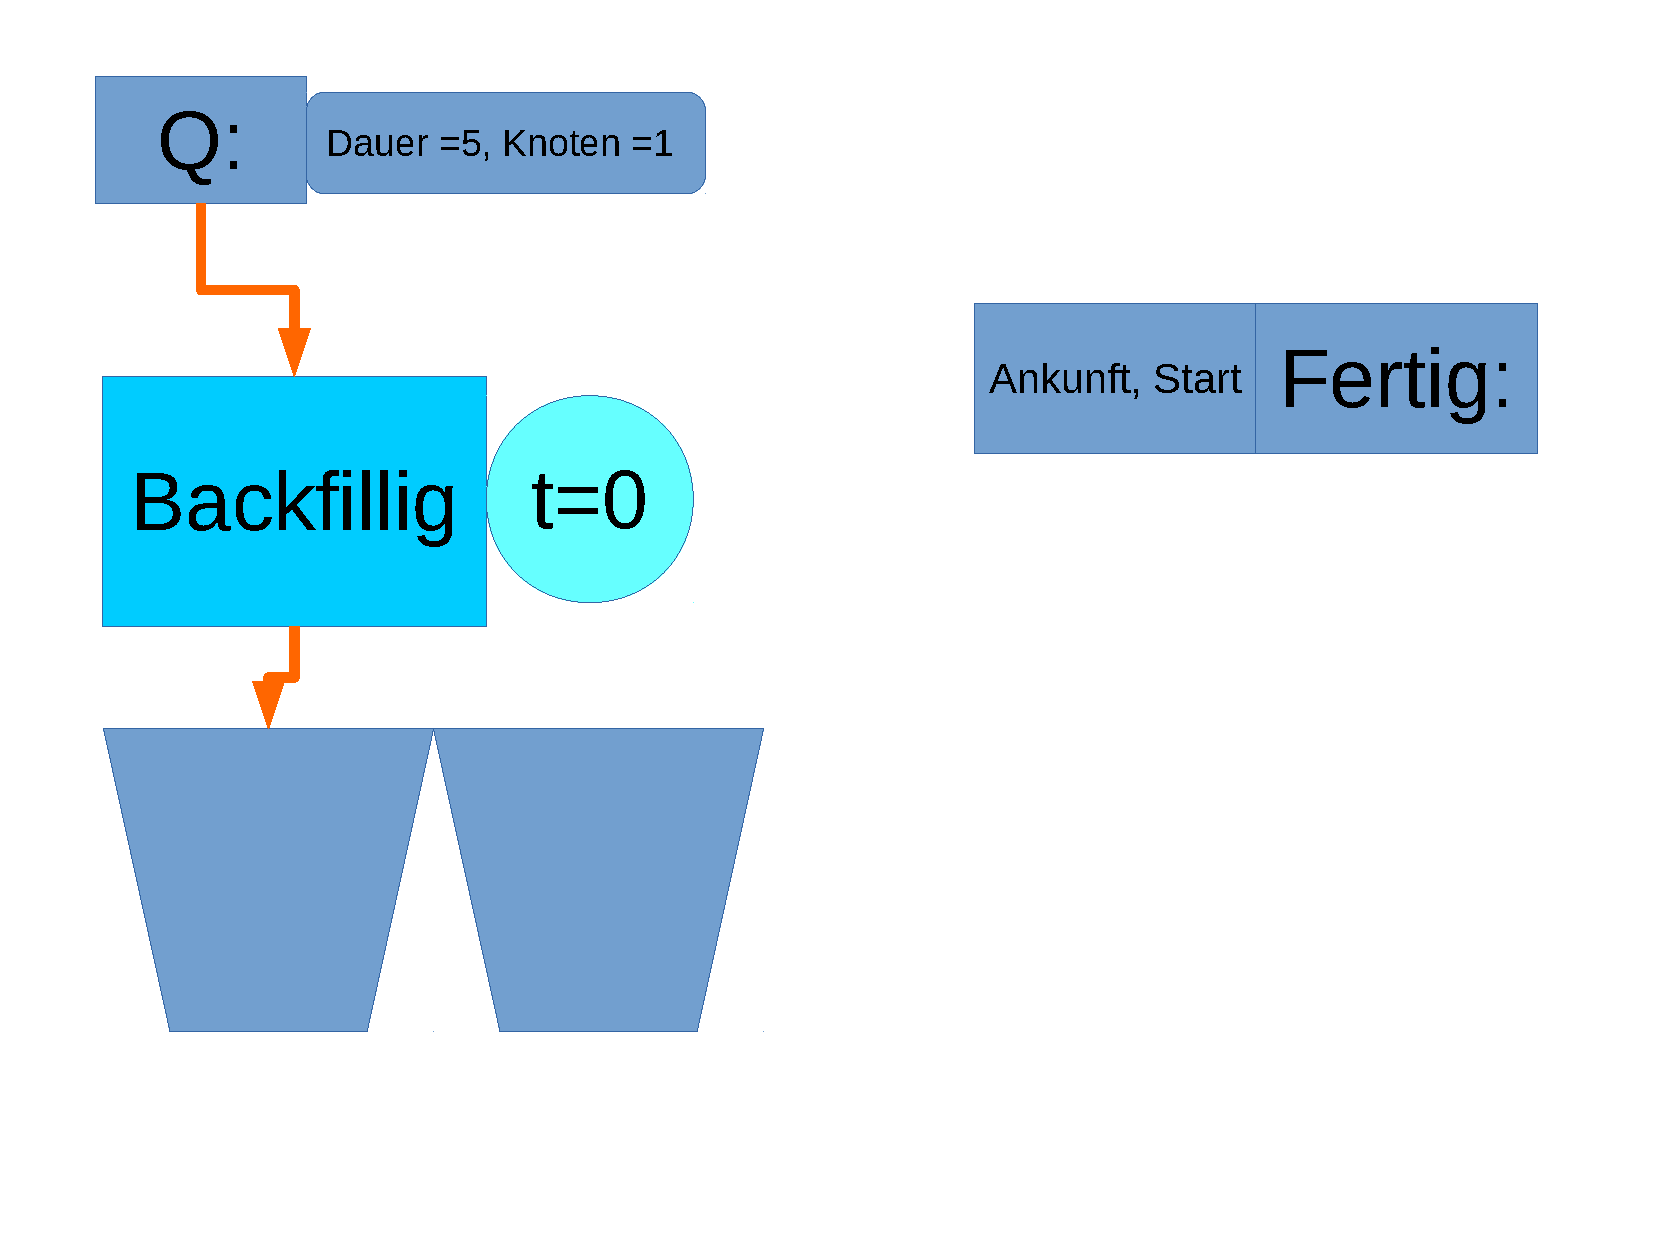
\includepdf[pages=-]{SchedulingBeispiel2.pdf}


%\section{Simulationsaufbau}
%\begin{frame}[t, fragile]{Simulations Paradigma\footnote{Matloff, Norm: Introduction to discrete-event simulati-
%		on and the simpy language. In: Davis, CA. Dept of Com-
%		puter Science. University of California at Davis. Retrieved on
%		August 2 (2008), Nr. 2009, S. 1–33}}
%	\begin{itemize}
%		\item Aktivit\"atsorientiert (Wettersystem, Physik Simulation in Videospielen)
%		\item \alert{Ereignisorientiert} (Fahrplan)
%		\item Prozessorientiert (Parallele Programmierung)
%	\end{itemize}
%\end{frame}

\begin{frame}[t, fragile]{Simulation und Auswertung}
	\begin{itemize}
		\item Arndt et al. \alert{designen 10 Experimente}, um unterschiedliches Verhalten der Algorithmen zu demonstrieren
		\item Variieren einen Parameter und vergleichen gew\"ahlte Zielfunktionen
		\item ''Bester Algorithmus'' wird \alert{qualitativ} bestimmt. Make span am wichtigsten
	\end{itemize}
\end{frame}

\begin{frame}[fragile]{Beispiel}

\begin{columns}
	\begin{column}{0.57\paperwidth}
		\vspace{0.5pt}
		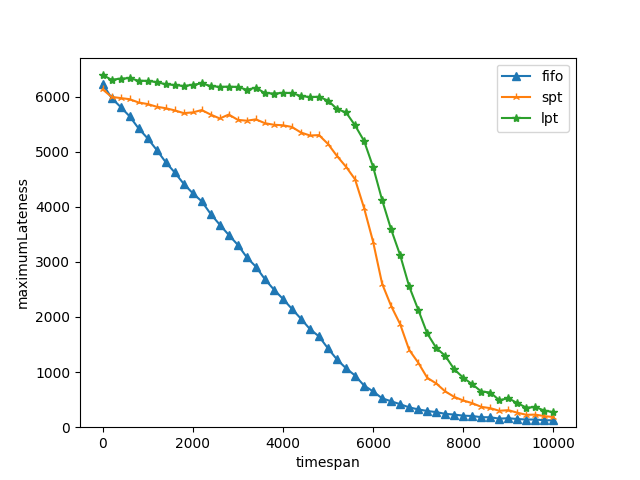
\includegraphics[width=\linewidth, clip]{images/Figure_2_2}
	\end{column}
	\begin{column}[c]{0.43\paperwidth}
		\begin{itemize}
			\item 250 Auftr\"age,1-50 k s Bearbeitungszeit
			\item 10 Knoten
			\item timespan - Sp\"atester Ankunftszeitpunkt wird variiert
			\item Mittel von 100 L\"aufen
		\end{itemize}
	\end{column}
\end{columns}
\end{frame}

\section{Eigene Untersuchungen}

\begin{frame}[t,fragile]{Optimistic Backfilling}
	W\"ahle den am l\"angsten wartenden Auftrag, falls startbar. Sonst w\"ahle einen Auftrag, der terminiert, bevor FiFo startet, ODER einen Auftrag, der weniger Knoten ben\"otigt, als \"ubrig bleiben werden, wenn FiFo startet.
\end{frame}

\begin{frame}[t,fragile]{Optimistic Backfilling Nachteil?}
\begin{itemize}[<+->]
	\item Gibt es einen Fall, in dem sich dies negativ auf die maximum lateness auswirkt?
	\item \begin{verbatim}
	Is fifo\_optimistic allways better than
	fifo\_backfill by maximumLateness?
	No! counterexample:
	queueintT, processingT, realProcessingT, degreeOfParallelism
	id: 0, qT: 1, pT: 3, rPT: 3, doP: 1
	id: 1, qT: 0, pT: 3, rPT: 3, doP: 2
	id: 2, qT: 0, pT: 1, rPT: 1, doP: 2
	id: 3, qT: 0, pT: 1, rPT: 1, doP: 3
	\end{verbatim}
\end{itemize}
\end{frame}

\begin{frame}[t,fragile]{Optimistic Backfilling Nachteil?}
\small
\begin{verbatim}	
	queueintT, processingT, realProcessingT, degreeOfParallelism
	id: 0, qT: 1, pT: 3, rPT: 3, doP: 1
	id: 1, qT: 0, pT: 3, rPT: 3, doP: 2
	id: 2, qT: 0, pT: 1, rPT: 1, doP: 2
	id: 3, qT: 0, pT: 1, rPT: 1, doP: 3

	maximumLateness of fifo\_optimistic: 4
	[0]:112|-3
	[1]:112|-3
	[2]:-00|03
	
	maximumLateness of fifo\_backfill: 3
	[0]:112|3--|-
	[1]:11-|300|0
	[2]:--2|3--|-
\end{verbatim}
\end{frame}

\begin{frame}[t,fragile]{Optimistic Backfilling Nachteil?}
	\begin{itemize}[<+->]
		\item make span Konservatives Backfilling 29\% l\"anger
		\item 4 Auftr\"age, 1 davon online, 3 Knoten
		\item Konservativ schlechter Optimistisch:\\
		4 Auftr\"age, 2 davon online, 3 Knoten
		\item Kompliziertere Konstellationen sind (vermutlich) seltener
		\item Vergleich mit Simulation: In ein paar Folien
	\end{itemize} 
\end{frame}

\begin{frame}[t, fragile]{Konservativ vs Optimistisch}
	\begin{itemize}
		\item Utilization and Predictability in Scheduling the IBM SP2 with Backfilling
		\footnote{Feitelson, Dror G. ; Weil, Ahuva M.: Utilization and pre-
			dictability in scheduling the IBM SP2 with backfilling. In:
			Proceedings of the First Merged International Parallel Proces-
			sing Symposium and Symposium on Parallel and Distributed
			Processing IEEE, 1998, S. 542–546}:\\
		''Results are that the performance (...) are practically identical''
		\item Attacking the bottlenecks of backfilling schedulers\footnote{Keleher, Peter J. ; Zotkin, Dmitry ; Perkovic, Dejan: At-
			tacking the bottlenecks of backfilling schedulers. In: Clus-
			ter Computing 3 (2000), Nr. 4, S. 245–254}:\\
		''This implies that there is significant difference between normalized distributions of job runtime estimates, and actual
		running times.''
	\end{itemize}
\end{frame}

\begin{frame}[t,fragile]{Gegenbeispiele Automatisch Finden}
	\begin{itemize}
		\item \alert{Anschauliche} Beispiele, in denen verschd. Algorithmen verschd. Entscheidungen treffen, helfen Intuition aufzubauen
		\item Idealerweise ''For Free'' aus dem Simulationsmodell ableitbar, ohne das Modell zu \"ubersetzten 
		\item L\"osung: \alert{Property Based Testing}
	\end{itemize}
\end{frame}
\begin{frame}[t,fragile]{Property Based Testing \footnote{Hughes, John ; Claessen, Koen: Quickcheck: a light-
		weight tool for random testing of haskell programs. In:
		Proceedings of the Fifth ACM SIGPLAN International Confe-
		rence on Functional Programming, ICFP, 2000, S. 268–279}}
	\begin{itemize}
		\item Eigenschaft einer Funktion, die immer gelten soll
		\item Zuf\"allige Eingaben ausprobiert, bis Eigenschaft verletzt wird
		\item Beispiel verkleinern (shrinking) 
	\end{itemize}
\end{frame}

\begin{frame}[t, fragile]{Beispiel}
\begin{itemize}

	\item Funktion: \emph{reverse}
	\item Eigenschaft: $reverse(x) == x$
	\item Zuf\"allige Eingaben: [] , [1], [2,2], [4,2]\lightning
	\item Verkleinern: 2 M\"oglichkeiten: Element l\"oschen oder Element verkleinern. 
	\item Verkleiern (l\"oschen): [4,2] $\rightarrow$ [4] \lightning
	\item Element Verkleinern: [4,2] $\rightarrow$ [1,2] $\rightarrow$ ... $\rightarrow$ [0,1]
\end{itemize}
\end{frame}

\begin{frame}[t, fragile]{Neue M\"oglichkeiten}
\begin{itemize}
	\item Testen der Implementation: FiFo nie besser als Konservatives Backfilling
	\item Beliebig Eigenschaften Aufbauen: besser nach mehreren Zielfunktionen.
	\item Monotonit\"at: System trifft bessere Entscheidungen, mit mehr Informationen: Fr\"uhere Ankuntszeiten $\implies$ nicht schlechtere Performance
	\item Schneller Aufbau von Intuition bez. neuer Algorithmen
\end{itemize}
\end{frame}

\begin{frame}[t, fragile]{Neue Algorithmen}
\begin{itemize}
	\item ''-Fit'': Smallest-Fit, Greatest-Fit
	\item Backfilling: Smallest-Backfill, Greatest-Backfill
	\item Optimistisches Backfilling nach Smallest,Greatest
	\item Backfilling nach zwei Funktionen; W\"ahle besten Kandidaten nach Funktion 1, falls nicht startbar, w\"ahle nach Funktion 2, ohne besten Kandidaten zu benachteiligen
	\item Analog f\"ur Optimistisches Backfilling
\end{itemize}
\end{frame}
\begin{frame}[t, fragile]{Vergleich mit Simulation}
	\begin{columns}
		\begin{column}{0.5\paperwidth}
			\vspace{0.5pt}
			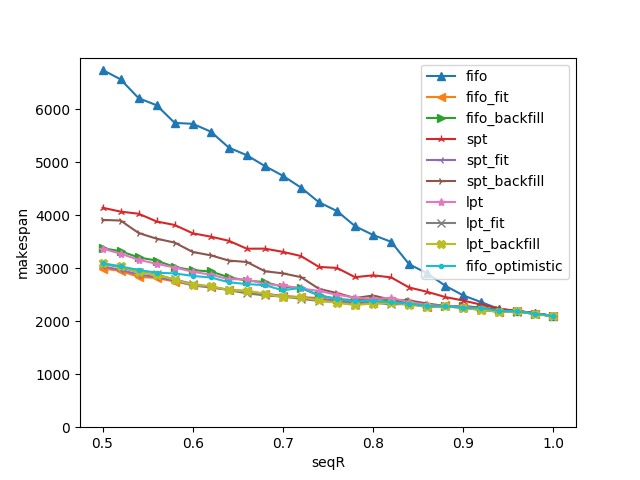
\includegraphics[width=\linewidth, clip]{images/Figure_5_1}
		\end{column}
		\begin{column}[c]{0.5\paperwidth}
			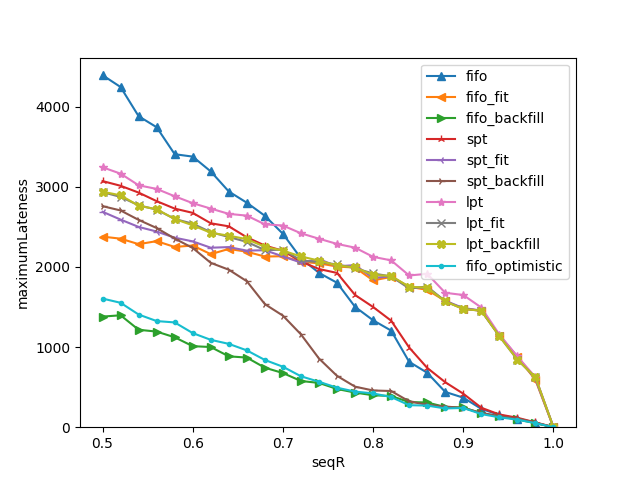
\includegraphics[width=\linewidth, clip]{images/Figure_5_2}
		\end{column}
	\end{columns}
\end{frame}

\begin{frame}[t,fragile]{Qualitative Analyse nicht mehr M\"oglich}
	\begin{itemize}
		\item In allen Kombinationen 80 Scheduling Algorithmen
		\item Zu jedem Ergebnis l\"asst sich ein passendes Experiment finden
		\item Algorithmen ohne konkretes Experiment vergleichen?
	\end{itemize}
\end{frame}

\begin{frame}[fragile]{PBT-Score}
		\vspace{0.5pt}
		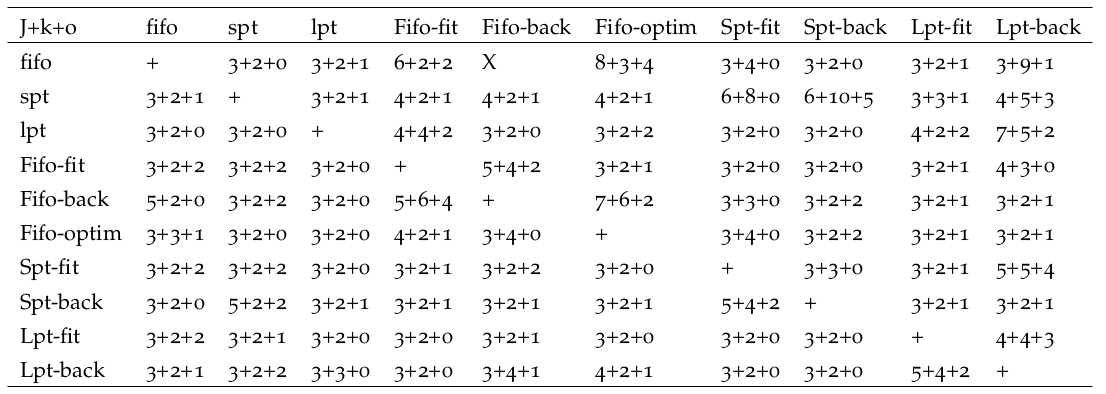
\includegraphics[width=\linewidth, clip]{images/SchedulerX.png}
\end{frame}
\begin{frame}[fragile]{PBT-Score\footnote{Rangkorrelations nach Spearman: -0.92 wenn mit Experiment 6 von Artndt et al. verglichen}}
\vspace{0.5pt}
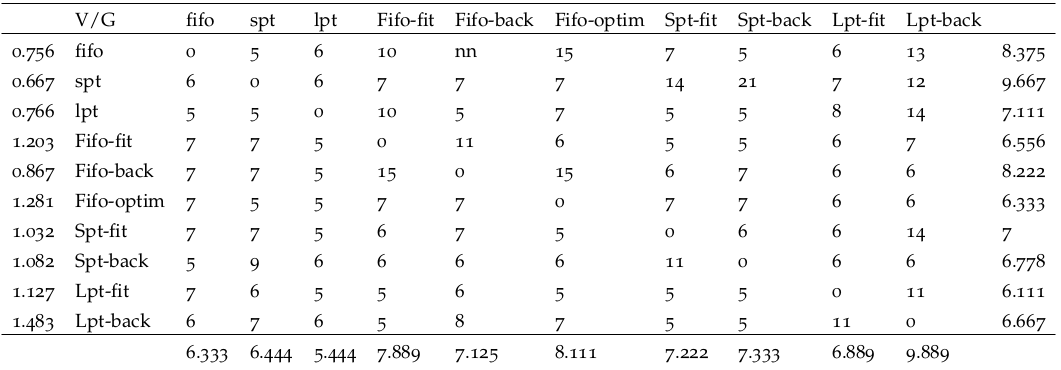
\includegraphics[width=\linewidth, clip]{images/SchedulerXScore.png}
\end{frame}

\section{Konklusion}
\begin{frame}[t,fragile]{Konklusion}
	\begin{itemize}
		\item Funktionale Sichtweise n\"utzlich
		\item PBT n\"utzlich, (fast) umsonst
		\item Zu jedem Ergebnis ist ein Experiment generierbar
		\item Deshalb problematisch, Algorithmen in beliebigen Situationen zu vergleichen
		\item Experimente m\"ussen aus der Realit\"at abgeleitet werden
		\item Algorithmen k\"onnen ohnke konkreten Fall verglichen werden
	\end{itemize}
\end{frame}

%-------------------------------------------
\end{document}
